% Figure 2: the pipeline of a transfer, where each failure class enters, and where limits sit.
% Gray ladder of hz_figstyle (0.10 / 0.42 / 0.68); Times to match IEEEtran; cards with a solid
% shadow. Compile: pdflatex fig_pipeline.tex
\documentclass[border=3pt]{standalone}
\usepackage{amsmath}
\usepackage{mathptmx}
\usepackage{tikz}
\usetikzlibrary{positioning, arrows.meta, calc}

\definecolor{ink}{gray}{0.10}
\definecolor{mid}{gray}{0.42}
\definecolor{light}{gray}{0.68}
\definecolor{fill}{gray}{0.955}

\tikzset{
  stage/.style={draw=ink, line width=0.7pt, fill=white, rounded corners=2pt,
                minimum width=1.86cm, minimum height=1.05cm, align=center, font=\footnotesize, inner sep=2pt},
  shadow/.style={fill=light, rounded corners=2pt, minimum width=1.86cm, minimum height=1.05cm},
  flow/.style={-{Stealth[length=5pt]}, line width=0.8pt, draw=ink},
  enter/.style={-{Stealth[length=4.5pt]}, line width=0.7pt, draw=mid},
  failure/.style={font=\footnotesize, text=ink, align=center, inner sep=1pt},
  limit/.style={draw=ink, line width=0.7pt, fill=fill, rounded corners=1.5pt, font=\footnotesize,
                align=center, minimum width=1.86cm, inner sep=2.5pt},
  covers/.style={font=\footnotesize, text=mid, align=center, inner sep=1pt},
}

\begin{document}
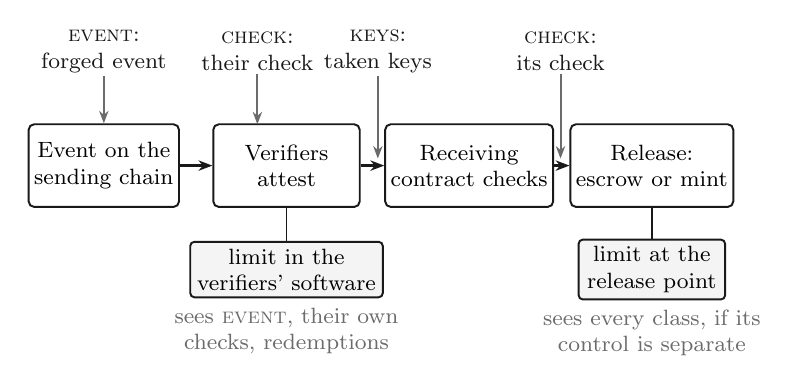
\begin{tikzpicture}
  \node[stage] (s1) at (0, 0) {Event on the\\sending chain};
  \node[stage] (s2) at (2.32, 0) {Verifiers\\attest};
  \node[stage] (s3) at (4.64, 0) {Receiving\\contract checks};
  \node[stage] (s4) at (6.96, 0) {Release:\\escrow or mint};
  \draw[flow] (s1) -- (s2);
  \draw[flow] (s2) -- (s3);
  \draw[flow] (s3) -- (s4);

  % where each failure class enters: an EVENT failure before the verifiers; a CHECK failure after the
  % check that failed, in the verifiers' own software or in the receiving contract; a KEYS failure after
  % the verifiers (valid attestations from taken keys)
  \node[failure] (fS) at (0, 1.45) {\textsc{event}:\\forged event};
  \node[failure] (fC1) at (1.95, 1.45) {\textsc{check}:\\their check};
  \node[failure] (fV) at (3.48, 1.45) {\textsc{keys}:\\taken keys};
  \node[failure] (fD) at (5.80, 1.45) {\textsc{check}:\\its check};
  \draw[enter] (fS) -- (s1.north);
  \draw[enter] (fC1) -- (1.95, 0.525);
  \draw[enter] (fV) -- (3.48, 0.09);
  \draw[enter] (fD) -- (5.80, 0.09);

  % where limits sit and which failures they see
  \node[limit] (lV) at (2.32, -1.32) {limit in the\\verifiers' software};
  \node[limit] (lR) at (6.96, -1.32) {limit at the\\release point};
  \draw[line width=0.6pt, draw=ink] (lV.north) -- (s2.south);
  \draw[line width=0.6pt, draw=ink] (lR.north) -- (s4.south);
  \node[covers, below=0.08cm of lV, align=center] {sees \textsc{event}, their own\\checks, redemptions};
  \node[covers, below=0.08cm of lR, align=center] {sees every class, if its\\control is separate};
\end{tikzpicture}
\end{document}
